\documentclass[11pt,a4paper]{article}

\usepackage[utf8]{inputenc}
\usepackage[T1]{fontenc}
\usepackage{amsmath,amssymb,amsfonts,mathtools}
\usepackage{booktabs}
\usepackage{array}
\usepackage[margin=1in]{geometry}
\usepackage{enumitem}
\usepackage{graphicx}
\usepackage{siunitx}
\usepackage{microtype}
\usepackage[hyphens]{url}
\usepackage[section]{placeins}

\newcommand{\dd}{\,\mathrm{d}}
\newcommand{\R}{\mathbb{R}}
\DeclareMathOperator{\tanhx}{tanh}
\DeclareMathOperator{\clamp}{clamp}

\title{\bfseries Hybrid ETAS Ranking of Earthquake Hazard in T\"urkiye}

\author{Bar{\i}\c{s} K{\i}s{\i}r\\
\small Independent Researcher, T\"urkiye}

\date{October 10, 2026}

\begin{document}
\maketitle

\begin{abstract}
Seismicity separates into two well-studied statistical regimes: short-scale
aftershock clustering, described by Epidemic-Type Aftershock-Sequence (ETAS)
point processes, and long-scale magnitude--frequency regularity, described by
the Gutenberg--Richter law. This paper specifies a deterministic,
catalogue-only forecasting engine that converts these regularities into
\emph{relative} regional hazard rankings over T\"urkiye and neighbouring
tectonic provinces (latitudes $34^\circ$--$43^\circ$N, longitudes
$24^\circ$--$46^\circ$E) on a $0.5^\circ$ grid. Four layers are combined:
an ETAS spatio-temporal field with a kernel-smoothed background and a fully
evaluated triggering kernel; a Gutenberg--Richter layer for completeness,
$b$-value mapping, and magnitude scaling; six bounded seismicity indicators;
and a Brownian-Passage-Time renewal layer for M$\ge$6 and M$\ge$7
recurrence. A threshold-dependent composite score blends the layers with
magnitude-specific weights and is normalised to a bounded display scale for
the M5+, M6+, and M7+ targets. Every equation is stated together with its
numerical constants and illustrated with worked examples computed from the
implementation itself; two figures are derived directly from the production
catalogue and three from the archived forecast snapshots. Because each
forecast uses only events at or before its calculation date, a bundled
archive of precomputed snapshots supports exact retrospective
reconstruction. Scores are within-catalogue relative rankings, never
occurrence probabilities, and the system carries standing messaging that it
is not a warning system.
\end{abstract}

\clearpage
\tableofcontents
\clearpage

\section{Introduction}
The Anatolian plate is squeezed westward between the Eurasian plate to the
north and the Arabian and African plates to the south and southwest. Its
northern boundary, the right-lateral North Anatolian Fault Zone (NAFZ), and
its southeastern boundary, the left-lateral East Anatolian Fault Zone (EAFZ),
have each hosted destructive magnitude-7 sequences, including the 1999
\.Izmit earthquake (M$_{\mathrm{w}}7.6$) on the NAFZ. Dense instrumental
coverage since the 2000s records tens of thousands of locatable events per
year in the broader region, which makes T\"urkiye a natural laboratory for
statistical earthquake forecasting: the catalogue is large, the tectonics are
localised onto major fault systems, and the observational history is long
enough to calibrate both clustering and renewal models.

Earthquake forecasting occupies a deliberate middle ground between two
extremes. Exact prediction of the time, place, and magnitude of individual
shocks is beyond current observational capability. At the other extreme,
time-independent hazard maps describe where large events are possible in
principle but say nothing about the current state of the system. Operational
forecasting, as codified for example by Jordan and co-workers
\cite{jordan2011} and tested continuously by the Collaboratory for the Study
of Earthquake Predictability \cite{ziemer2022}, assigns expected activity
rates that evolve as new data arrive and submits them to prospective,
like-for-like testing. The engine described here belongs to this tradition
but narrows its claims further: it outputs rankings of regions rather than
calibrated rates, on the argument that a transparent ordering of signals is
more honest than a probability number whose calibration has not been earned.

The recent literature sharpens the case for a strong classical baseline.
Neural point-process models evaluated on chronological earthquake forecasting
benchmarks have repeatedly failed to outperform a well-specified ETAS model
\cite{stockman2026, epbench2025}, while hybrid convolutional-recurrent
architectures are judged precisely by whether they pass the same CSEP test
suite as ETAS \cite{cl-etas2023}. The implication is that the marginal value
of additional complexity must be demonstrated against ETAS, not assumed. The
present engine therefore keeps ETAS at its centre and adds only bounded,
interpretable modifiers whose individual contributions can be read off the
composite score term by term.

Three design decisions organise the work:

\begin{enumerate}[label=\textbf{(D\arabic*)},leftmargin=2.6em]
  \item \textbf{Catalogue-only computation.} No waveform, geodetic, or
  learned model state enters the evaluation; every score is a deterministic
  function of the merged instrumental and historical catalogue and a
  reference timestamp.
  \item \textbf{Threshold-dependent composition.} The M5+, M6+, and M7+
  rankings emphasise different processes---aftershock clustering for M5+,
  balanced evidence for M6+, long-term loading for M7+---through separate
  weight vectors, so the three maps are genuinely different orderings rather
  than rescalings of one field.
  \item \textbf{Explicit non-probability scoring.} Display scores live on a
  bounded $[40,99]$ scale produced by per-ranking min--max normalisation, and
  the product states plainly that they are relative ranks rather than
  occurrence probabilities.
\end{enumerate}

Section~\ref{sec:data} describes the catalogue and its growth.
Section~\ref{sec:methods} states the full computational specification with
worked examples. Section~\ref{sec:product} presents the forecast product and
its map figures. Section~\ref{sec:eval} defines the evaluation diagnostics,
and Section~\ref{sec:discussion} the limitations.

\section{Data and Catalogue Construction}\label{sec:data}

\subsection{Source and shards}
The source is the Sismik Harita earthquake-list API
(\texttt{sismikharita.com/api}), which merges agency feeds (notably EMSC and
TURHEC) with historical compilations. The repository bundles the catalogue as
immutable JSON shards: one accumulation shard for pre-2000 events and one
shard per year for $2000$--$2026$, totalling about \SI{1.23e6}{events} in
roughly \SI{1.0}{GiB}. The 2026-08-01 forecast snapshot, for reference, was
computed from $1{,}230{,}423$ events with the newest event dated
2026-07-31T23:56:42Z. Each record carries an occurrence timestamp (UTC),
latitude, longitude, magnitude, depth, a review label, the number of
contributing agencies, the inter-source magnitude spread, and a
primary-record flag. Records with unparseable or future timestamps,
non-finite coordinates, or non-finite magnitudes are discarded, and the rest
are clipped to the study rectangle.

\subsection{Catalogue growth and completeness drift}
Figure~\ref{fig:annual} plots the annual in-region event counts recovered
from the $2000$--$2026$ shards. Two facts stand out. First, yearly totals
grew roughly tenfold, from $4{,}286$ events in 2000 (17 at M5+) to $59{,}138$
in 2025 (36 at M5+), reflecting denser networks and broader agency merging
rather than a tenfold change in Earth behaviour. Second, individual years
carry the imprint of productive sequences: 2011 ($38{,}776$ events), 2020
($43{,}247$ events, 50 at M5+), and 2023 ($92{,}214$ events, 59 at M5+) each
stand well above their neighbours because aftershock cascades contribute
large numbers of locatable small events. Both facts motivate the rolling
calibration design of Section~\ref{sec:mc}: a fixed absolute time window
would mix very different detection regimes, so completeness, $b$-value, and
background rate are re-estimated on a trailing ten-year window at every
evaluation.

\begin{figure}[h]
\centering
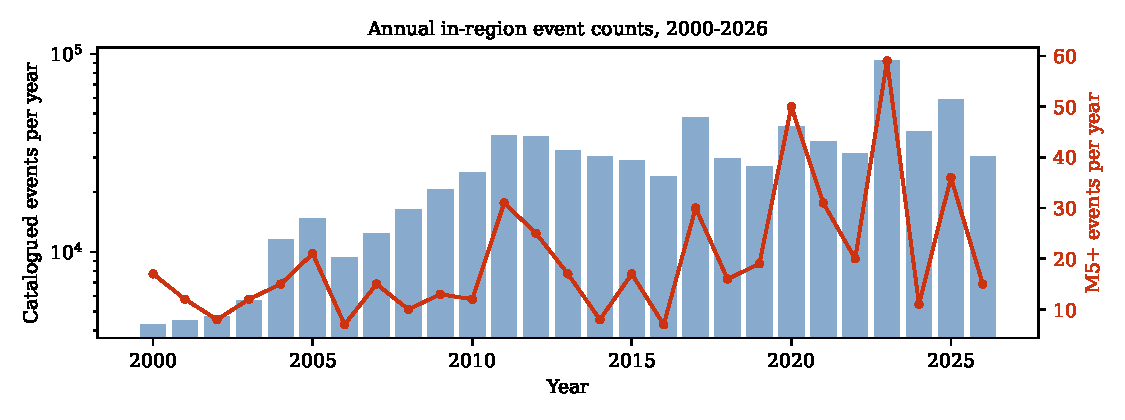
\includegraphics[width=0.85\linewidth]{figures/fig1_annual_counts.pdf}
\caption{Annual in-region event counts from the bundled shards, 2000--2026
(left axis, logarithmic bars), with M5+ counts overlaid (right axis, line).
The secular rise records improving detection; the spikes in 2011, 2020, and
2023 record highly productive sequences. The 2026 bar is a partial year.}
\label{fig:annual}
\end{figure}

\subsection{Snapshot archive and calculation dates}
A distinctive property of the system is that history is reproducible. Because
the engine is deterministic and consumes only events at or before a chosen
cut-off, the repository bundles $363$ precomputed forecast snapshots
(\texttt{data/snapshots/*.json}) covering millennial milestones, every year
$1900$--$2026$, and the elapsed months of the current year. A
calculation-date selector maps each user-facing option to a bundle key: a
month option \texttt{YYYY-MM} of the current year resolves to the first of
that month; a standalone year $1900$--$2026$ resolves to January 1 of that
year; pre-1900 range labels resolve to their range-start year; and the
current calendar day resolves to itself. The exclusive UTC cut-off for a key
is the start of that date when the day field is $01$ (so a year snapshot
contains strictly the events before January 1) and the end of that date
otherwise (so the current-day snapshot contains everything known). Serving a
historical selection therefore never recomputes: it reads the matching
bundle, and any option missing from the archive is rejected rather than
computed on demand.

\subsection{Daily update pipeline}
Once per T\"urkiye calendar day (UTC+3), at the first request after
midnight, the server refreshes the catalogue from the provider starting
$48$ hours before the newest stored event. The overlap captures late
arrivals and revisions; stale ranges are split into windows of at most $28$
days; incoming records are normalised, de-duplicated by stable identity, and
merged keeping the latest revision of each event. Forecast results are cached
in memory, in temporary files, and in object storage under unique candidate
names, with readers selecting the candidate of greatest catalogue coverage so
that concurrent serverless instances cannot overwrite a complete result with
a stale one.

\subsection{Observation-quality weights}\label{sec:quality}
Every prepared event carries a quality weight $w\in[0.1,1.0]$ that
multiplies its contribution throughout the pipeline. The review label sets a
base weight,

\begin{equation}
w_{\text{base}} =
\begin{cases}
1.00 & \texttt{reviewed},\ \texttt{focal\_mechanism}\\
0.90 & \texttt{turhec\_extended}\\
0.74 & \texttt{preliminary}\\
0.62 & \texttt{automatic}\\
0.48 & \texttt{historical\_catalogue}\\
0.82 & \text{otherwise},
\end{cases}
\end{equation}

where \texttt{preliminary} denotes the provider's label for preliminary,
unreviewed solutions. The final weight is

\begin{equation}
w = \clamp\Big(w_{\text{base}}\cdot f_{\text{src}}\cdot f_{\text{spread}}
\cdot f_{\text{depth}}\cdot f_{\text{primary}},\;0.1,\;1.0\Big),
\end{equation}

with agency factor
\begin{equation}
f_{\text{src}}=\clamp(0.94+0.03\min(s_{\text{cnt}},3),\,0.94,\,1.03)
\end{equation}
and spread penalty
\begin{equation}
f_{\text{spread}}=\clamp(1.04-0.22\,\sigma_M,\,0.68,\,1.04)
\end{equation}
applied when a spread is reported; $f_{\text{depth}}=0.5$ for depths outside
$[0,700]$\,km and $1$ otherwise; and $f_{\text{primary}}=0.5$ for non-primary
duplicate records and $1$ otherwise. Two worked examples fix the arithmetic. A reviewed event from
two agencies with spread $0.2$ receives
$1.00\times1.00\times0.996=0.9960$. An automatic single-agency event with
spread $0.5$ receives $0.62\times0.97\times0.93=0.5593$. Implausible depths
and duplicate records are therefore down-weighted but never silenced
entirely, since even a doubtful record carries some information.

\section{Methods}\label{sec:methods}
The engine is a pure function of (catalogue, reference timestamp). It runs
once per T\"urkiye day to build an immutable base field, from which the full
method$\times$threshold$\times$count matrix is derived without shared mutable
state. What follows states each stage exactly, with the constants used by the
implementation and worked numerical examples.

\subsection{Grid geometry}
The domain is a regular $0.5^\circ$ grid with

\begin{align}
\phi_{\min}=34^\circ,\ \phi_{\max}=43^\circ,\qquad
\lambda_{\min}=24^\circ,\ \lambda_{\max}=46^\circ,
\end{align}

giving $N_\phi=\lceil9/0.5\rceil=18$ rows, $N_\lambda=\lceil22/0.5\rceil=44$
columns, and $N_{\text{cells}}=792$ cells in row-major order. Row $r$ is
centred at $\bar\phi_r=34+(r+\tfrac12)0.5$ and column $c$ at
$\bar\lambda_c=24+(c+\tfrac12)0.5$. Cell area corrects for meridian
convergence with $k=111.195$\,km\,deg$^{-1}$:

\begin{equation}
A_{\text{cell}}(r)=(\Delta\phi\cdot k)\cdot(\Delta\lambda\cdot k\cdot
\cos\bar\phi_r).
\end{equation}

As an example, at $\bar\phi=38.25^\circ$ the area is
$55.5975^2\times\cos38.25^\circ=3091.7\times0.78528=2427.48$\,km$^2$; across
the domain the area ranges over roughly $2300$--$2700$\,km$^2$. Inner kernels
use the flat-Earth distance
$\dd r=\sqrt{(\Delta\lambda\,k\cos\bar\phi)^2+(\Delta\phi\,k)^2}$, accurate at
regional scales, while the recurrence geometry uses the exact haversine
distance.

\subsection{Event preparation}
Raw records are parsed to UTC epoch seconds, rejected on invalid or future
timestamps or non-finite coordinates or magnitudes, clipped to the rectangle,
and assigned quality weights per Section~\ref{sec:quality}, yielding prepared
events $\{(\tau_i,\varphi_i,\lambda_i,M_i,w_i)\}$.

\subsection{Magnitude of completeness}\label{sec:mc}
Calibration uses the trailing $W_{\text{cal}}=10$ years of prepared events
(the full catalogue only when fewer than $200$ events remain), binned at
$\Delta m=0.1$ over $100$ bins. Two estimators are combined. Maximum
curvature (MAXC) takes the mode bin $m^*$ of the non-cumulative distribution
and adds a conservative half-bin correction,
$M_{\mathrm{MAXC}}=m^*\Delta m+0.2$ \cite{weimer2000}. Goodness-of-fit at 95
percent (GFT95) scans trial magnitudes $2.0$--$3.2$ (requiring at least $200$
events above trial) and accepts the smallest trial whose fitted G--R line
reproduces cumulative counts within $5$ percent relative absolute error:

\begin{equation}
1-\frac{\sum_{k}\left|\Delta N^{\text{obs}}_k-\hat N(M_k)\right|}
{\sum_k\Delta N^{\text{obs}}_k}\ge0.95,\qquad
\hat N(M_k)=N_{\ge M_{\text{trial}}}10^{-b(M_k-M_{\text{trial}})}.
\end{equation}

Completeness is the conservative envelope
$M_c=\max(M_{\mathrm{MAXC}},M_{\mathrm{GFT95}})$ clamped to $[2.0,3.2]$,
falling back to MAXC alone when GFT95 admits no candidate. A secondary
$\Delta a$ estimator after Godano and Petrillo scans trial thresholds and
takes the first at which the G--R $a$-value jumps by more than
$\min(\Delta a)+0.3$; it is implemented for offline analysis.

Figure~\ref{fig:fmd} applies these exact estimators to the $2016$--$2025$
annual shards ($430{,}859$ in-region events). The non-cumulative mode bin is
$13$ (magnitude $1.3$), so MAXC gives $1.5$, which the floor clamp raises to
$2.00$; GFT95 independently returns $2.0$. Hence $M_c=2.00$ with
$N_{\ge M_c}=148{,}464$ and mean magnitude $1.81$. The fitted G--R line in
panel (b) uses the $b$-value of the next section. The lesson is instructive
rather than alarming: a modern dense catalogue detects vast numbers of
micro-earthquakes, and the clamp floor keeps the analysis safely above the
detection roll-off.

\begin{figure}[h]
\centering
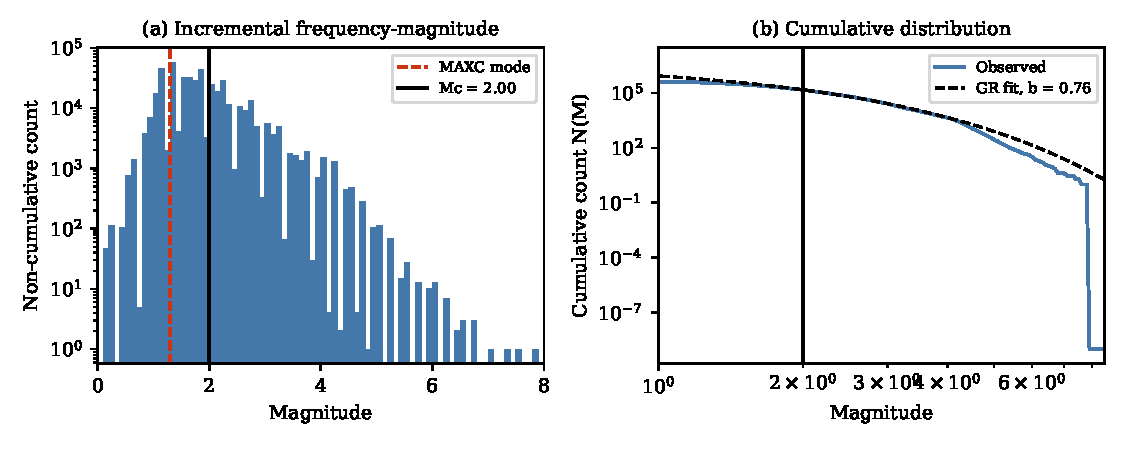
\includegraphics[width=0.9\linewidth]{figures/fig2_fmd_magnitude.pdf}
\caption{Frequency--magnitude distribution of the 2016--2025 in-region events
($n=430{,}859$). (a) Non-cumulative counts per $0.1$ bin with the MAXC mode
(dashed) and the adopted $M_c=2.00$ (solid). (b) Cumulative counts with the
fitted G--R line at $b=0.76$. Both estimators agree at the clamp floor.}
\label{fig:fmd}
\end{figure}

\subsection{Gutenberg--Richter layer}\label{sec:gr}
The global $b$-value is the Aki--Utsu maximum-likelihood estimate
\cite{aki1965} over events with $M\ge M_c$,

\begin{equation}
b_{\text{global}}=\frac{\log_{10}e}
{\langle M\rangle-(M_c-\Delta m/2)},
\quad\text{clamped to }[0.6,1.4],
\label{eq:bvalue}
\end{equation}

with fallback $0.9$ below $100$ qualifying events. On the Figure~\ref{fig:fmd}
data, $\langle M\rangle=1.8143$ is not directly comparable because the mean
there spans all magnitudes; restricted to $M\ge2.00$ the estimator yields
$b=0.7577$. The $a$-value $a=\log_{10}N_{\ge M_c}+bM_c$ gives
$a=\log_{10}(148464)+0.7577\times2.0=5.17157+1.51540=6.68702$, and the
expected maximum magnitude $M_{\max}^{\mathrm{GR}}=a/b=8.8254$, clipped to
$[M_c+0.3,8.5]$ where an upper bound is required.

Spatially varying $b$-values pool all $M\ge M_c$ events in each cell's
$3\times3$ neighbourhood ($1.5^\circ\times1.5^\circ$) and apply
Equation~\eqref{eq:bvalue} with the global $M_c$; cells with fewer than $100$
pooled events receive no local estimate. The non-negative anomaly
$\Delta b=\max(0,b_{\text{global}}-b_{\text{local}})$ marks relatively
stressed neighbourhoods \cite{scholz1968,gulia2019}. Rates at $M_c$ are
extrapolated to a target threshold by
$S(M_{\mathrm{thr}})=10^{-b(M_{\mathrm{thr}}-M_c)}$ with the local $b$ where
available. For $b=1.0$ and $M_c=2.6$ the factors are
$S(5)=3.981072\times10^{-3}$, $S(6)=3.981072\times10^{-4}$, and
$S(7)=3.981072\times10^{-5}$: each magnitude unit costs exactly one order of
magnitude in rate, which is why the three thresholds rank different cells.

\subsection{Declustering}
The background field admits only independent events. Gardner--Knopoff (1974)
windows \cite{gardner1974} are applied in one chronological sweep with a
rolling active-parent list:

\begin{align}
\Delta t_{\mathrm{GK}}(M)&=
\begin{cases}
10^{\,0.5409\,M-0.547}, & M<6.5,\\
10^{\,0.032\,M+2.7389}, & M\ge6.5,
\end{cases}
\quad\text{(days)},\\
\Delta r_{\mathrm{GK}}(M)&=10^{\,0.1238\,M+0.983}
\quad\text{(km)}.
\end{align}

An event not larger than a still-active parent and inside \emph{both} of its
windows is flagged as dependent; survivors become parents in turn. Concrete
window sizes: M5.0 spans $143.71$ days and $39.99$\,km; M6.0 spans
$499.34$ days and $53.19$\,km; M6.5 spans $884.91$ days and $61.33$\,km; M7.8
spans $973.87$ days and $88.85$\,km. The kink at M6.5 is part of the
published parameterisation, not an implementation choice. Stochastic EM
declustering \cite{zhuang2002} is noted as a future replacement.

\subsection{Background intensity}
The background rate at each cell centre is the quality-weighted Gaussian
density over declustered events, normalised by the complete span
$T_{\text{cal}}$ in days \cite{helmstetter2007}:

\begin{equation}
\mu(\mathbf{x}_c)=\frac{A_{\text{cell}}(r)}{2\pi h^2}\,
\frac{1}{T_{\text{cal}}}\sum_{j\in\mathcal{B}}
w_j\,\exp\!\Big(-\frac{r_{jc}^2}{2h^2}\Big),
\label{eq:mu}
\end{equation}

with $h=25$\,km. The units are expected independent events per cell per day
at $M_c$. A worked example: one unit-quality event at a cell centre with
$A_{\text{cell}}=2427.48$\,km$^2$ and $T_{\text{cal}}=3650$ days contributes
$2427.48/(2\pi\times625)/3650=1.693568\times10^{-4}$ per day. Scaled to M5+
with $b=0.7577$ and $M_c=2.0$, the factor is $10^{-0.7577\times3.0}
=5.332121\times10^{-3}$, giving an annual M5+ rate of $3.298254\times10^{-4}$
whose base-ten logarithm is $-3.4817$---the quantity that enters the
composite score of Section~\ref{sec:composite}. A $3.5^\circ\times4.5^\circ$
bounding box keeps the $O(N_{\text{cells}}\times\lvert\mathcal{B}\rvert)$
evaluation tractable.

\subsection{Triggered intensity}\label{sec:trig}
The triggered rate sums the separable ETAS kernel over all $M\ge M_c$ events
at the reference time $t$,

\begin{equation}
\lambda_{\mathrm{trig}}(\mathbf{x}_c,t)=
\sum_{i\,:\,t_i<t}k(M_i)\;g(t-t_i)\;f\big(r_{ic},M_i\big),
\label{eq:triggered}
\end{equation}

with the three factors below (Figure~\ref{fig:kernels} shows their shapes).

\begin{figure}[h]
\centering
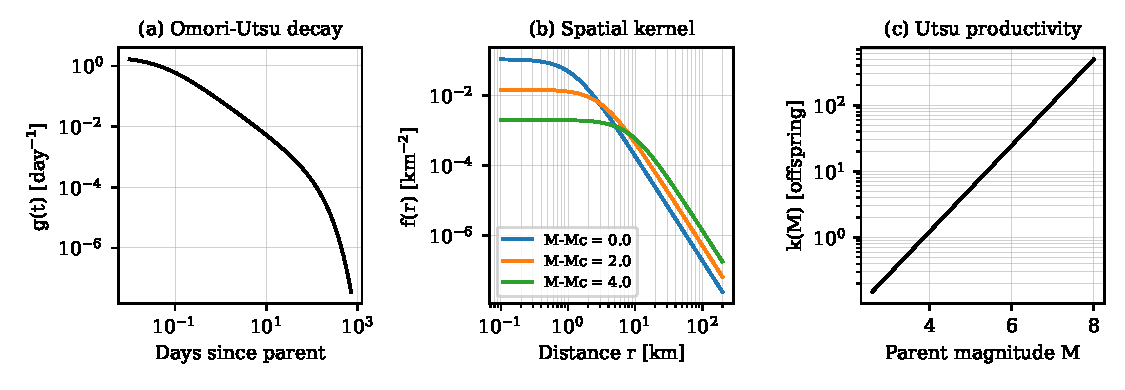
\includegraphics[width=0.95\linewidth]{figures/fig3_etas_kernels.pdf}
\caption{The three ETAS kernel factors at production parameters.
(a) Omori--Utsu density $g(\Delta t)$ with $c=0.05$\,d, $p=1.1$,
$\tau=100$\,d. (b) Spatial density $f(r)$ for magnitude excess
$M-M_c\in\{0,2,4\}$ above $M_c=2.6$. (c) Utsu productivity $k(M)$ with
$K=0.15$, $\alpha=1.5$.}
\label{fig:kernels}
\end{figure}

\emph{Utsu productivity.} The expected direct-offspring count is
$k(M)=K\exp(\alpha(M-M_c))$ with $K=0.15$ and $\alpha=1.5$. At $M_c=2.6$:
$k(3.0)=0.2733$, $k(5.0)=5.4897$, $k(6.0)=24.6033$, $k(7.0)=110.2643$,
$k(7.8)=366.0903$. Because the form is exponential in the excess, ratios
depend only on magnitude differences: $k(7)/k(5)=\exp(1.5\times2)=20.0855$.
An optional dual-productivity scheme (Zhang et al., 2020; disabled by
default) assigns $\alpha_{\text{short}}=2.0$ to the most recent
$h\,10^{-bM_c}$ events ($h=2\times10^5$) and $\alpha_{\text{long}}=1.4$ to
older ones.

\emph{Omori--Utsu decay.} The tapered temporal density is

\begin{equation}
g(\Delta t)=\frac{p-1}{c}\Big(1+\frac{\Delta t}{c}\Big)^{-p}
\exp\!\Big(-\frac{\Delta t}{\tau}\Big),\qquad
c=0.05\ \text{d},\ p=1.1,\ \tau=100\ \text{d},
\end{equation}

in days$^{-1}$, normalised to unit integral without the taper. Evaluated:
$g(0)=2.0$, $g(0.5)=0.1423399$, $g(1)=0.06954178$, $g(7)=0.008062846$,
$g(30)=0.001300109$, $g(365)=2.925058\times10^{-6}$,
$g(730)=3.546986\times10^{-8}$. The taper removes the $t\to0$ singularity
from numerical reach and imposes finite memory; residual mass beyond $730$
days is about $6.2\times10^{-6}$, which justifies truncating the sum there.
Combined with productivity, an M6.0 parent contributes a space-integrated
$24.6033\times0.06954178=1.710957$ events per day one day after the shock,
falling to $24.6033\times0.001300109=0.031987$ per day after thirty days.

\emph{Spatial kernel.} Offspring spread as the power law

\begin{align}
f(r,M)&=\frac{q-1}{\pi\,d(M)^2}
\left(1+\frac{r^2}{d(M)^2}\right)^{-q},\qquad q=1.5,\\
d(M)&=D_0\,\exp\!\big(\gamma\,(M-M_c)\big),\qquad
D_0=1.2\ \text{km},\ \gamma=0.5,
\end{align}

with $d(M)$ clamped to $[1,400]$\,km and unit integral over $\R^2$. At
$M=M_c$ ($d=1.2$\,km): $f(0)=1.105243\times10^{-1}$,
$f(10\,\text{km})=1.869337\times10^{-4}$,
$f(50\,\text{km})=1.526568\times10^{-6}$ per km$^2$. At excess $2.0$
($d=3.2619$\,km): $1.495783\times10^{-2}$, $4.460938\times10^{-4}$,
$4.126854\times10^{-6}$. At excess $4.0$ ($d=8.8669$\,km):
$2.024323\times10^{-3}$, $5.911400\times10^{-4}$,
$1.077728\times10^{-5}$. Per-cell weights multiply by cell area, clamp to
$1$, and renormalise across touched cells per parent, so narrow kernels keep
their mass on a coarse grid.

\subsection{Threshold scaling}
For $M_{\mathrm{thr}}\in\{5,6,7\}$ the total daily rate is
\begin{equation}
\lambda_{\text{total}}(M_{\mathrm{thr}})=
\big[\mu(\mathbf{x}_c)+\lambda_{\mathrm{trig}}(\mathbf{x}_c,t)\big]
\,10^{-b\,(M_{\mathrm{thr}}-M_c)},
\end{equation}
annualised by $365.2425$. The clustering ratio is
\begin{equation}
\rho=\frac{\lambda_{\mathrm{trig}}}{\mu+\lambda_{\mathrm{trig}}},
\end{equation}
which diagnoses how much of a cell's rate is triggered rather than
background.

\subsection{Seismicity indicators}
Indicators use a trailing $5$-year window (energy, CV, natural time, rate
change); $M_c$, $b$, and $\mu$ use $10$ years. Accumulation is per cell,
then pooled over $3\times3$ neighbourhoods.

\emph{Coefficient of variation.} Over inter-event gaps, requiring at
least $3$ gaps \cite{kagan1991,corral2004},
\begin{equation}
\mathrm{CV}=\frac{\sigma_{\Delta t}}{\mu_{\Delta t}},\qquad
\sigma^2_{\Delta t}=
\frac{\sum_k\delta_k^2-(\sum_k\delta_k)^2/n}{\,n-1\,}.
\end{equation}
Example: gaps $[10,12,9,40]$ days give mean
$17.75$, sample deviation $14.89$, and $\mathrm{CV}=0.8386$ (near-periodic);
gaps $[1,2,1,60]$ give mean $16.0$, deviation $29.34$, and
$\mathrm{CV}=1.8336$ (strongly clustered).

\emph{Root-energy rate.} With $\log_{10}E=1.5M+4.8$ \cite{hanks1979},
$\sqrt{E_i}=10^{0.75M_i+2.4}$ and
$\dd E^{1/2}/\dd t=T_{\text{ind}}^{-1}\sum_i\sqrt{E_i}$ in
J$^{1/2}$\,yr$^{-1}$. Reference values: M3.0 releases $1.9953\times10^9$\,J
($\sqrt{E}=4.4668\times10^4$); M5.0 releases $1.9953\times10^{12}$\,J
($1.4125\times10^6$); M6.0 releases $6.3096\times10^{13}$\,J
($7.9433\times10^6$); M7.0 releases $1.9953\times10^{15}$\,J
($4.4668\times10^7$). The indicator measures released energy, never stored
energy.

\emph{Natural-time progress.} With $M_S=3.0$ and $M_T=5.0$
\cite{rundle2016,rundle2021}, $N_{\mathrm{GR}}=10^{b(M_T-M_S)}$ and
$\pi_{\mathrm{nt}}=1-\exp(-n/N_{\mathrm{GR}})$, where $n$ counts small events
since the last local target reset. For $b=1.0$, $N_{\mathrm{GR}}=100$, and
$n=0,20,50,100,200,400$ give progress $0.000000$, $0.181269$, $0.393469$,
$0.632121$, $0.864665$, $0.981684$. Cells without any past target event
receive no value. This is a G--R-normalised proxy, not an empirical
probability.

\emph{Rate-change $z$.} Habermann's statistic \cite{habermann1987} with
$T_{\text{rec}}=365$ days,
\begin{equation}
z=\frac{r_{\text{rec}}-r_{\text{long}}}{\sqrt{r_{\text{long}}/T_{\text{rec}}}},
\qquad
r_{\text{rec}}=\frac{N_{\text{rec}}}{T_{\text{rec}}},\quad
r_{\text{long}}=\frac{N_{\text{long}}}{T_{\text{ind}}}.
\end{equation}
Example: $12$ events in
the recent year against $80$ in five years gives
$r_{\text{rec}}=0.032877$, $r_{\text{long}}=0.043806$, and $z=-0.9981$,
mild quiescence. The value is reported but excluded from the composite
score after quarterly checks showed no stable skill for the next $90$-day
M5+ outcome.

\emph{Magnitude deficit.} $\Delta M=M_{\max}^{\mathrm{GR}}-M_{\max}^
{\mathrm{obs}}$ clamped to $[-1,5]$, diagnostic only. On the
Figure~\ref{fig:fmd} numbers, $M_{\max}^{\mathrm{GR}}=8.8254$, so a cell
whose observed maximum is $7.8$ reports $\Delta M=1.0254$.

\subsection{Large-event recurrence}\label{sec:bpt}
Mainshocks with $M\ge6$ are separately declustered, sequence-collapsed
(minimum gaps $2$ years for M6+, $3$ years for M7+), and collected within
$75$\,km (M6+) or $110$\,km (M7+) neighbourhoods; fewer than three
independent mainshocks yields no value rather than zero. Sample intervals
give mean $\bar\delta$ and aperiodicity shrunk toward the prior $0.6$ with
prior size $3$, clamped to $[0.35,1]$. The Brownian Passage Time density,
CDF, and $30$-year conditional probability are

\begin{align}
f_{\mathrm{BPT}}(t;\mu,\alpha)&=
\sqrt{\frac{\mu}{2\pi\alpha^2t^3}}\,
\exp\!\Big[-\frac{(t-\mu)^2}{2\mu\alpha^2t}\Big],\\
F_{\mathrm{BPT}}(t)&=\Phi(u_1)+e^{2/\alpha^2}\,\Phi(-u_2),\qquad
u_{1,2}=\frac{\sqrt{t/\mu}\mp\sqrt{\mu/t}}{\alpha},\\
P_{30}^{\mathrm{BPT}}&=
\frac{F_{\mathrm{BPT}}(t_e+30)-F_{\mathrm{BPT}}(t_e)}
{1-F_{\mathrm{BPT}}(t_e)},
\end{align}

with $\Phi$ by the Abramowitz--Stegun approximation (error below
$7.5\times10^{-8}$) \cite{matthews2002,wgcep2003}. Worked example with mean
recurrence $100$ years, aperiodicity $0.6$, and $80$ elapsed years:
$F(80)=0.457689$ and $F(110)=0.672629$, so that
\begin{equation}
P_{30}^{\mathrm{BPT}}=
\frac{0.672629-0.457689}{1-0.457689}=0.396341,
\end{equation}
against a Poisson baseline $1-e^{-30/100}=0.259182$. The renewal memory
thus raises
the conditional probability by more than half relative to the memoryless
model at this elapsed fraction. The reported probability blends BPT with
Poisson by confidence
$\kappa=\clamp(n_{\text{int}}/6,0,1)\cdot(0.5+0.5\bar w)$,
$P_{30}=\kappa P_{30}^{\mathrm{BPT}}+(1-\kappa)[1-e^{-30/\bar\delta}]$,
scored as $P_{30}(0.5+0.5\kappa)$.

\subsection{Centroids}
Reporting positions are decay-weighted mean epicentres with weights
\begin{equation}
w_{\text{cen}}=w_i\cdot10^{0.3(M_i-M_c)}\cdot
e^{-\,\text{age}_i/15\ \text{yr}}.
\end{equation}
Example: a unit-quality M6.0 event at $M_c=2.6$ seen two years ago carries
$10^{1.02}\times e^{-2/15}=10.471\times0.8752=9.1642$, so large recent
events dominate the centroid while old small ones fade.

\subsection{Composite score}\label{sec:composite}
The cell score blends the log-annual rate with bounded indicator terms and a
magnitude-feasibility term:

\begin{align}
H_{\text{cell}}=&\ \log_{10}\!\big(\lambda^{\text{ann}}+\varepsilon\big)
+\ln\!\big[f_{\text{feas}}(M_{\mathrm{thr}},M_{\max}^{\mathrm{obs}})\big]
\nonumber\\
&+w_b\,\clamp\!\Big(\frac{\Delta b}{b_{\text{global}}},0,0.5\Big)
+w_{\mathrm{nt}}\,\clamp\!\big(\pi_{\mathrm{nt}}-0.5,\,-0.5,\,0.5\big)
\nonumber\\
&+w_{\mathrm{en}}\,\tanhx\!\Big(\frac{\dd E^{1/2}/\dd t}{10^9}\Big)
+w_{\mathrm{cv}}\,\clamp\!\Big(\frac{\mathrm{CV}-1}{2},\,0,\,1\Big)
\nonumber\\
&+w_{\mathrm{rec}}\,P_{30}\,\big(0.5+0.5\kappa\big),
\label{eq:composite}
\end{align}

with $\varepsilon=10^{-12}$ and

\begin{equation}
f_{\text{feas}}(M_{\mathrm{thr}},M_{\max})=
\exp\!\Big[-\frac{\max(0,M_{\mathrm{thr}}-M_{\max})^2}{2\cdot(0.8)^2}\Big].
\end{equation}

Feasibility is a soft Gaussian penalty, never a hard cut, because a finite
catalogue cannot prove an unobserved magnitude impossible. For a cell with
$M_{\max}^{\mathrm{obs}}=5.3$: $f_{\text{feas}}(5)=1.000000$ ($\ln=0.0000$),
$f_{\text{feas}}(6)=0.681941$ ($\ln=-0.3828$),
$f_{\text{feas}}(7)=0.104579$ ($\ln=-2.2578$). The M7+ ranking therefore
discounts such a cell by $2.26$ score units before any indicator is
considered, which is the main reason the three thresholds order cells
differently. Every modifier is bounded, so no outlier can dominate.

\begin{table}[h]
\centering
\caption{Composite-score weights by magnitude threshold.}
\label{tab:weights}
\begin{tabular}{lcccc}
\toprule
Weight & M5+ & M6+ & M7+ & Dominant rationale\\
\midrule
$w_b$ (b-value anomaly) & 0.03 & 0.07 & 0.14 & long-term stress accumulation\\
$w_{\mathrm{nt}}$ (natural time) & 0.05 & 0.09 & 0.14 & long-cycle progress\\
$w_{\mathrm{en}}$ (energy rate) & 0.04 & 0.06 & 0.10 & released-energy activity\\
$w_{\mathrm{cv}}$ (clustering) & 0.12 & 0.06 & 0.02 & aftershock clustering (M5+)\\
$w_{\mathrm{rec}}$ (recurrence) & 0.00 & 0.50 & 1.00 & long-term repeat history\\
\bottomrule
\end{tabular}
\end{table}

\subsection{Selection and normalisation}
Candidates sort by composite score and survive greedily only when at least
$1.8$ cell widths (about $100$\,km) from every accepted cell, so one
aftershock zone cannot occupy the whole list. The $50$ survivors are min--max
normalised,

\begin{equation}
s_{\text{disp}}=40+59\cdot
\frac{H_{\text{cell}}-H_{\min}}{H_{\max}-H_{\min}}\in[40,99],
\end{equation}

and banded at $\ge92$ (very high), $\ge80$ (high), $\ge65$ (notable), and
below (elevated). Example: with pool extremes $-6.2$ and $-2.1$, a cell at
$-3.0$ maps to $40+59\times3.2/4.1=86.0488$, reported as $86.0$ (high). The
display score is a within-ranking position, not a probability.

\subsection{Single-signal methods}
The same field yields eight single-signal orderings: Poisson
($\log_{10}\mu^{\text{ann}}$), ETAS ($\log_{10}\lambda^{\text{ann}}$),
Triggered, b-value anomaly, natural time, energy, clustering, and historical
recurrence. Each is normalised independently and scores cannot be compared
across methods. The b-value, natural-time, energy, and clustering layers are
threshold-independent by construction.

\subsection{Parameter inventory}
Table~\ref{tab:params} collects every numerical constant for reproducibility
in one place; all symbols are defined in the sections above.

\begin{table}[h]
\centering
\caption{Complete numerical parameter inventory of the engine.}
\label{tab:params}
\begin{tabular}{lll}
\toprule
Symbol & Value & Role\\
\midrule
$\Delta\phi$ & $0.5^\circ$ & grid cell size\\
Domain & $34$--$43^\circ$N, $24$--$46^\circ$E & study rectangle\\
$N_{\text{cells}}$ & $18\times44=792$ & grid size\\
$k$ & $111.195$\,km\,deg$^{-1}$ & degree-to-km factor\\
$W_{\text{cal}}$ / $W_{\text{ind}}$ & $10$ / $5$ years & calibration / indicator windows\\
$\Delta m$, bins & $0.1$, $100$ & FMD binning\\
$M_c$ clamp & $[2.0,3.2]$, GFT $95$ percent & completeness envelope\\
$b$ clamp, $N_{\min}^{b}$ & $[0.6,1.4]$, $100$ events & G--R slope guard\\
$M_{\max}$ clip & $[M_c+0.3,8.5]$ & upper-bound guard\\
$h$ & $25$\,km & background bandwidth\\
$K$, $\alpha$ & $0.15$, $1.5$ & Utsu productivity\\
$c$, $p$, $\tau$ & $0.05$\,d, $1.1$, $100$\,d & Omori--Utsu decay\\
Lookback & $730$ days & trigger summation cap\\
$q$, $D_0$, $\gamma$ & $1.5$, $1.2$\,km, $0.5$ & spatial kernel\\
$d(M)$ clamp & $[1,400]$\,km & aftershock-zone guard\\
$T_{\text{rec}}$ & $365$ days & rate-change recent window\\
CV gaps & $\ge3$ & variation guard\\
$M_S$, $M_T$ & $3.0$, $5.0$ & natural-time counting levels\\
$\Delta M$ clamp & $[-1,5]$ & deficit guard\\
Recurrence radii & $75$\,km (M6+), $110$\,km (M7+) & neighbourhoods\\
Sequence gaps & $2$\,yr (M6+), $3$\,yr (M7+) & collapse rule\\
$\alpha_0$, clamp & $0.6$ prior, $[0.35,1]$ & aperiodicity guard\\
$H$ & $30$ years & recurrence horizon\\
Feasibility $\sigma$ & $0.8$ & magnitude-support width\\
Separation & $1.8$ cells & spatial de-duplication\\
Display range & $[40,99]$, pool $50$ & normalisation\\
Radii & $75$ / $120$ / $180$\,km & M5+ / M6+ / M7+ influence\\
\bottomrule
\end{tabular}
\end{table}

\subsection{Computational implementation}
Fields are \texttt{Float64Array} buffers of length $792$; per-event
characteristic radii and elapsed days are cached before the inner cell loop;
cosines of row latitudes are precomputed once; and both kernel summations
apply the $3.5^\circ\times4.5^\circ$ bounding box before any transcendental
evaluation. The background pass costs $O(N_{\text{cells}}\times
\lvert\mathcal{B}\rvert)$ and the triggered pass
$O(N_{\text{cells}}\times E_{730})$ with $E_{730}$ the events of the last
$730$ days, after which neighbourhood pooling is linear in the cell count.
No stage shares mutable state across thresholds or methods, and identical
inputs reproduce identical outputs bit-for-bit subject only to floating-point
determinism of a single thread.

\section{Forecast Product}\label{sec:product}
The dashboard renders the top-ranked signals on an interactive Leaflet map
(Figure~\ref{fig:ui}) with a method selector, a magnitude-threshold selector,
a signal-count selector, and the calculation-date selector of
Section~\ref{sec:data}. Each marker reports its rank, centroid, influence
radius, display score, signal band, and the full indicator suite, including
annualised background, triggered, and total rates, the clustering ratio,
$b$-value and completeness, quality-weighted counts, recency, energy rate,
CV, natural-time progress, rate-change $z$, magnitude deficit, and the
recurrence quadruple where defined.

\begin{figure}[h]
\centering
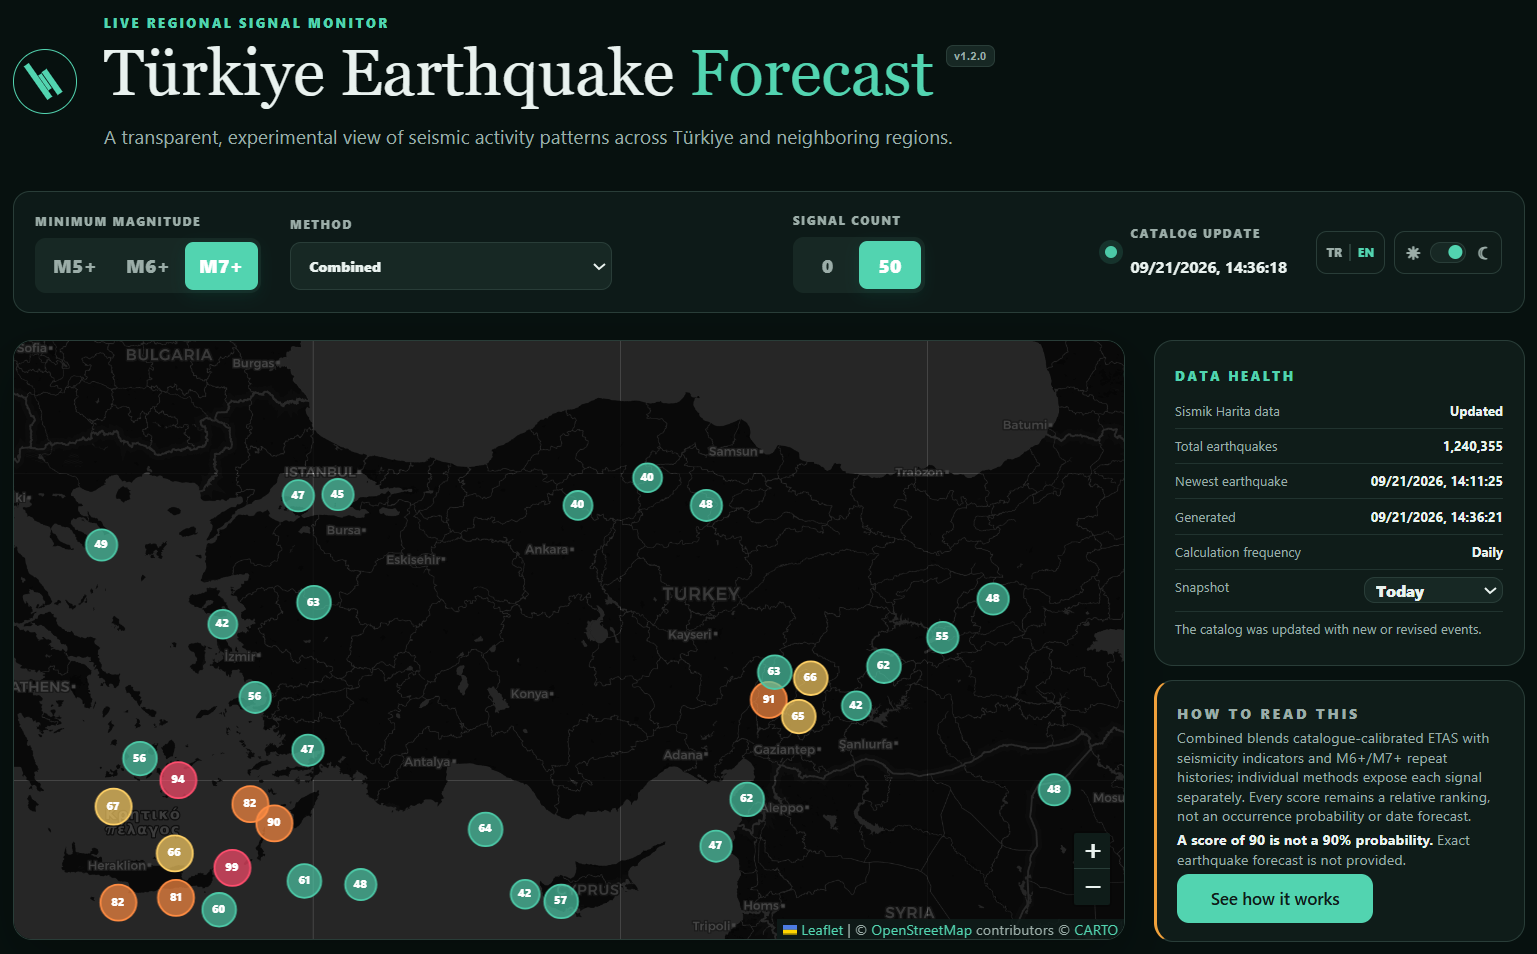
\includegraphics[width=0.72\linewidth]{figures/fig4_dashboard.png}
\caption{The interactive dashboard rendering the ranked signal field on a
Leaflet map. Marker size and colour encode the display score; the
calculation-date selector reproduces any archived historical field.}
\label{fig:ui}
\end{figure}

Figure~\ref{fig:map7} plots the archived combined-M7+ top $50$ of the
2026-08-01 snapshot over the model grid. The two highest cells score $99$
at $(34.82^\circ\text{N},25.30^\circ\text{E})$ in the Hellenic arc southwest
of Crete and at $(34.97^\circ\text{N},45.09^\circ\text{E})$ on the eastern
edge, followed by $85.1$ at $(35.36^\circ\text{N},27.15^\circ\text{E})$ and
$84.8$ at $(36.34^\circ\text{N},25.90^\circ\text{E})$; the schematic NAFZ
and EAFZ traces are drawn for orientation only. Figure~\ref{fig:thr} places
the M5+, M6+, and M7+ combined fields side by side from the same snapshot:
the orderings visibly differ, with M5+ emphasising Aegean and western
Anatolian clustering and M7+ concentrating on the Hellenic arc and the
eastern borderlands, exactly as the weight schedule of
Table~\ref{tab:weights} intends.

\begin{figure}[h]
\centering
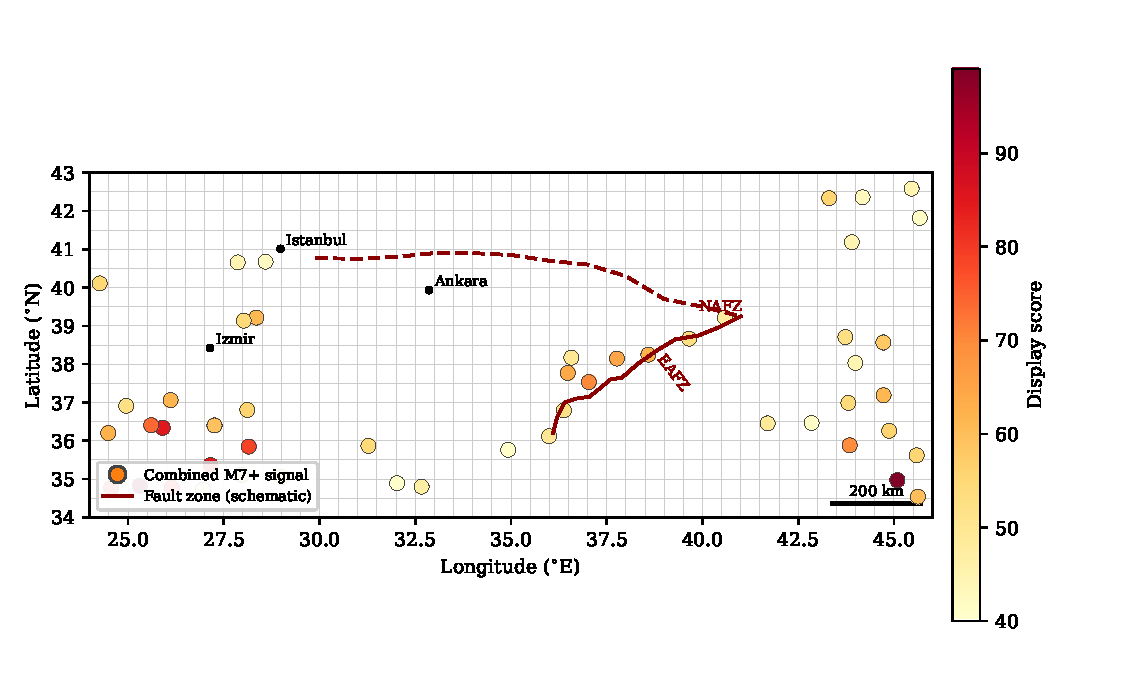
\includegraphics[width=0.95\linewidth]{figures/fig5_map_m7_snapshot.pdf}
\caption{Combined-M7+ top-50 ranking field from the 2026-08-01 snapshot
(catalogue cut-off 2026-07-31, $1{,}230{,}423$ events). Circle colour encodes
the display score on $[40,99]$; fault traces are schematic and shown for
orientation; the $200$\,km bar is computed at $38.5^\circ$N.}
\label{fig:map7}
\end{figure}

\begin{figure}[h]
\centering
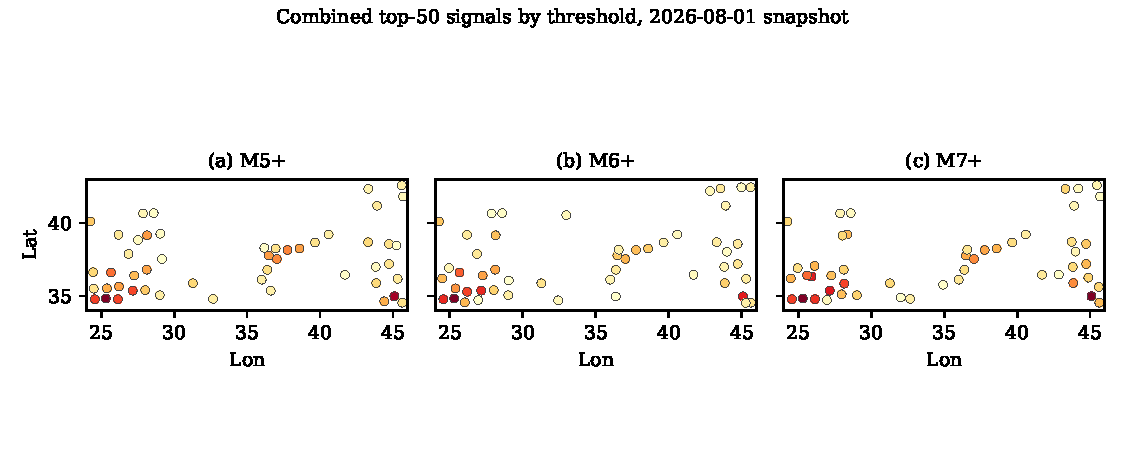
\includegraphics[width=0.95\linewidth]{figures/fig6_maps_thresholds.pdf}
\caption{Combined top-50 signals by target threshold from the same 2026-08-01
snapshot. The three orderings differ because feasibility, clustering, and
recurrence weights are threshold-dependent (Table~\ref{tab:weights}).}
\label{fig:thr}
\end{figure}

\section{Evaluation and Diagnostics}\label{sec:eval}
Offline testing uses CSEP-style primitives. The Poisson log-likelihood
drops the constant factorial term,
\begin{equation}
\mathcal{L}=\sum_i\big[y_i\log\lambda_i-\lambda_i\big],
\end{equation}
the information gain per event is
\begin{equation}
\mathrm{IGPE}=
\frac{\mathcal{L}_{\text{target}}-\mathcal{L}_{\text{ref}}}{N_{\text{obs}}},
\end{equation}
and the Brier score with its skill score is
\begin{equation}
\mathrm{BS}=\frac{1}{N}\sum_i(f_i-o_i)^2,\qquad
\mathrm{BSS}=1-\frac{\mathrm{BS}}{\mathrm{BS}_{\text{ref}}}.
\end{equation}
The monotone Poisson transform $P=1-e^{-\lambda H}$ applies for fixed
horizons. The accompanying
software studies report three retrospective findings that shaped the
production configuration. First, a chronological $2012$--$2025$
pseudo-prospective comparison of calibration windows found the $10$-year
background at mean M5+ spatial information gain $0.658$ per event over
$2019$--$2025$ against $0.442$ for $20$ years, with $3$-, $5$-, and
$10$-year indicator windows scoring $0.51126$, $0.51115$, and $0.51001$;
the differences among indicator windows are negligible and five years is
retained as the stable middle choice. Second, chronological $30$-year
holdouts of the recurrence layer reached mean cell-level AUC $0.697$ for
M6+ and $0.596$ for M7+, weak-to-moderate discrimination that justifies the
confidence blending and subordinate role of Section~\ref{sec:bpt}. Third,
quarterly pseudo-prospective checks of the rate-change $z$-value found no
stable discrimination for the following $90$-day M5+ outcome, which is why
$z$ and the magnitude deficit are reported but unscored. All figures are
retrospective and await prospective confirmation.

\section{Discussion and Limitations}\label{sec:discussion}
The engine is conservative by construction, and four limitations from the
earlier specification stand, joined here by three further qualifications.

First, completeness drift (Section~\ref{sec:data}) is mitigated by rolling
estimation but never removed; pre-1900 entries are sparse and detection has
improved tenfold within the instrumental era.

Second, Gardner--Knopoff declustering is a deterministic heuristic; the
background rate inherits its errors, and stochastic alternatives
\cite{zhuang2002} or time-varying completeness corrections
\cite{mizrahi2021} would improve $\mu$.

Third, the composite weights are fixed engineering values rather than
likelihood fits, so no occurrence probability is, or should be, derived
from the display score.

Fourth, nothing beyond the catalogue enters: fault geometry, slip rates,
geodetic locking, and stress transfer are absent, so the M7+ layer states
catalogue regularity, not physical constraint.

Fifth, the grid is coarse relative to rupture dimensions. An M7+ rupture
spans tens of kilometres \cite{wells1994}, comparable to a $0.5^\circ$ cell,
so near-field ranking cannot resolve along-strike variations; the
$1.8$-cell separation and the $75$--$180$\,km influence radii are explicit
acknowledgements of this resolution limit.

Sixth, all kernels are isotropic and depth-blind: directivity, fault
orientation, and the seismogenic thickness play no role, which flatters
circular aftershock zones over elongated ones.

Seventh, the daily cadence and the $730$-day trigger cap mean the model
responds to sequences within days but forgets them within years by design;
it is a ranking of the present state, not a memory of all history.

The standing disclaimer follows from these points: relative ranks, not
probabilities, and no use as a warning system.

\section{Conclusion}
This paper has stated, equation by equation and example by example, a
reproducible four-layer catalogue-only engine for ranking regional seismic
signals in T\"urkiye and neighbouring regions at M5+, M6+, and M7+
thresholds. Full ETAS spatio-temporal modelling, Gutenberg--Richter
completeness and $b$-value mapping, six bounded indicators, and a
Brownian-Passage-Time recurrence layer are composed with
threshold-dependent weights and normalised to a non-probabilistic display
scale; the parameter inventory, the worked examples, and the six figures fix
the behaviour completely. Prospective testing of the rankings against future
events is the natural next step.

\section*{Code and Data Availability}
The engine is open source under the MIT license. Repository:
\begin{center}
\url{https://github.com/bariskisir/TurkiyeEarthquakeForecast}
\end{center}
Live dashboard:
\begin{center}
\url{https://turkiyeearthquakeforecast.bariskisir.com}
\end{center}
Bundled catalogue shards and the $363$ precomputed forecast snapshots ship
with the repository; daily updates are retrieved from the Sismik Harita API
(\texttt{sismikharita.com/api}).

\section*{Acknowledgments}
The author thanks the Sismik Harita team for the public catalogue API and
the open seismology community whose software and parameterisations informed
this work. No external funding supported this study.

\FloatBarrier

\bibliographystyle{unsrt}
\begin{thebibliography}{99}

\bibitem{ogata1988} Ogata, Y. (1988). Statistical models for earthquake
occurrences and residual analysis for point processes. \emph{Journal of the
American Statistical Association}, 83(401), 9--27.

\bibitem{ogata1998} Ogata, Y. (1998). Space-time point-process models for
earthquake occurrences. \emph{Annals of the Institute of Statistical
Mathematics}, 50(2), 379--402.

\bibitem{utsu1961} Utsu, T. (1961). A statistical study on the occurrence of
aftershocks. \emph{Geophysical Magazine}, 30, 521--605.

\bibitem{gutenberg1944} Gutenberg, B., and Richter, C. F. (1944). Frequency
of earthquakes in California. \emph{Bulletin of the Seismological Society of
America}, 34(4), 185--188.

\bibitem{aki1965} Aki, K. (1965). Maximum likelihood estimate of $b$ in the
formula $\log N=a-bM$ and its confidence limits. \emph{Bulletin of the
Earthquake Research Institute}, 43, 237--239.

\bibitem{gardner1974} Gardner, J. K., and Knopoff, L. (1974). Is the sequence
of earthquakes in Southern California, with aftershocks removed, Poissonian?
\emph{Bulletin of the Seismological Society of America}, 64(5), 1363--1367.

\bibitem{weimer2000} Wiemer, S., and Wyss, M. (2000). Minimum magnitude of
completeness in earthquake catalogs: examples from Alaska, the western
United States, and Japan. \emph{Bulletin of the Seismological Society of
America}, 90(4), 859--869.

\bibitem{scholz1968} Scholz, C. H. (1968). The frequency--magnitude relation
of microfracturing in rock and its relation to earthquakes. \emph{Bulletin
of the Seismological Society of America}, 58(1), 399--415.

\bibitem{gulia2019} Gulia, L., and Wiemer, S. (2019). Real-time
discrimination of earthquake foreshocks and aftershocks. \emph{Nature}, 574,
193--199.

\bibitem{helmstetter2007} Helmstetter, A., Kagan, Y. Y., and Jackson, D. D.
(2007). High-resolution time-independent grid-based forecast for $M\ge5$
earthquakes in California. \emph{Seismological Research Letters}, 78(1),
78--86.

\bibitem{hanks1979} Hanks, T. C., and Kanamori, H. (1979). A moment magnitude
scale. \emph{Journal of Geophysical Research}, 84(B5), 2348--2350.

\bibitem{wells1994} Wells, D. L., and Coppersmith, K. J. (1994). New
empirical relationships among magnitude, rupture length, rupture width,
rupture area, and surface displacement. \emph{Bulletin of the Seismological
Society of America}, 84(4), 974--1002.

\bibitem{zhuang2002} Zhuang, J., Ogata, Y., and Vere-Jones, D. (2002).
Stochastic declustering of space-time earthquake occurrences. \emph{Journal
of the American Statistical Association}, 97(458), 369--380.

\bibitem{matthews2002} Matthews, M. V., Ellsworth, W. L., and Reasenberg,
P. A. (2002). A Brownian model for recurrent earthquakes. \emph{Bulletin of
the Seismological Society of America}, 92(6), 2233--2250.

\bibitem{wgcep2003} Working Group on California Earthquake Probabilities
(2003). Earthquake probabilities in the San Francisco Bay Region:
2002--2031. \emph{U.S. Geological Survey Open-File Report 03-214}.

\bibitem{rundle2016} Rundle, J. B., et al. (2016). Nowcasting earthquakes.
\emph{Earth and Space Science}, 3(11), 480--486.

\bibitem{rundle2021} Rundle, J. B., et al. (2021). Nowcasting earthquakes: a
comparison of induced earthquakes in Oklahoma and tectonic earthquakes.
\emph{Pure and Applied Geophysics}, 178, 2503--2518.

\bibitem{kagan1991} Kagan, Y. Y., and Jackson, D. D. (1991). Long-term
earthquake clustering. \emph{Geophysical Journal International}, 104(1),
117--133.

\bibitem{corral2004} Corral, A. (2004). Long-term clustering, scaling, and
universality in the temporal occurrence of earthquakes. \emph{Physical Review
Letters}, 92(10), 108501.

\bibitem{habermann1987} Habermann, R. E. (1987). Man-made changes of
seismicity rates. \emph{Bulletin of the Seismological Society of America},
77(1), 141--159.

\bibitem{asencio2016} Asencio-Cort\'es, G., et al. (2016). Earthquake
prediction in California using regression algorithms and cloud-based big
data infrastructure. \emph{Computers and Geosciences}, 115, 198--210.

\bibitem{wang2026} Wang, F., et al. (2026). A machine-learning framework with
parameter optimization and regional clustering for strong earthquake
prediction. \emph{Journal of Seismology}.

\bibitem{zhang2020} Zhang, Y., et al. (2020). Improved earthquake forecasting
model based on long-term memory in earthquakes. \emph{arXiv:2003.12539}.

\bibitem{jordan2011} Jordan, T. H., et al. (2011). Operational earthquake
forecasting: state of knowledge and guidelines for utilization. \emph{Annals
of Geophysics}, 54(4), 315--391.

\bibitem{ziemer2022} Ziemer, S., et al. (2022). Collaboratory for the Study
of Earthquake Predictability: statistical evaluation of forecasts.
\emph{Seismological Research Letters}.

\bibitem{mizrahi2021} Mizrahi, L., Nandan, S., and Wiemer, S. (2021).
Embracing data incompleteness for better earthquake forecasting.
\emph{Journal of Geophysical Research: Solid Earth}, 126(12),
e2021JB022379.

\bibitem{nandan2019} Nandan, S., et al. (2019). Forecasting the full
distribution of earthquake numbers is fair, robust, and better.
\emph{Seismological Research Letters}, 90(4), 1650--1659.

\bibitem{brehmer2026} Brehmer, J., et al. (2026). Enhancing the statistical
evaluation of earthquake forecasts. \emph{arXiv preprint}.

\bibitem{stockman2026} Stockman, S., et al. (2026). EarthquakeNPP:
benchmarking neural point processes for earthquake forecasting.
\emph{Transactions on Machine Learning Research}.

\bibitem{epbench2025} Stockman, S., et al. (2025). EPBench: a global
short-term earthquake prediction benchmark. \emph{arXiv preprint}.

\bibitem{cl-etas2023} Zhang, S., et al. (2023). CL-ETAS: combining
convolutional LSTM with ETAS for earthquake forecasting. \emph{arXiv
preprint}.

\end{thebibliography}

\end{document}